\documentclass[tikz, border=1cm]{standalone}

\usepackage{tikz}
\usetikzlibrary{calc}

\begin{document}
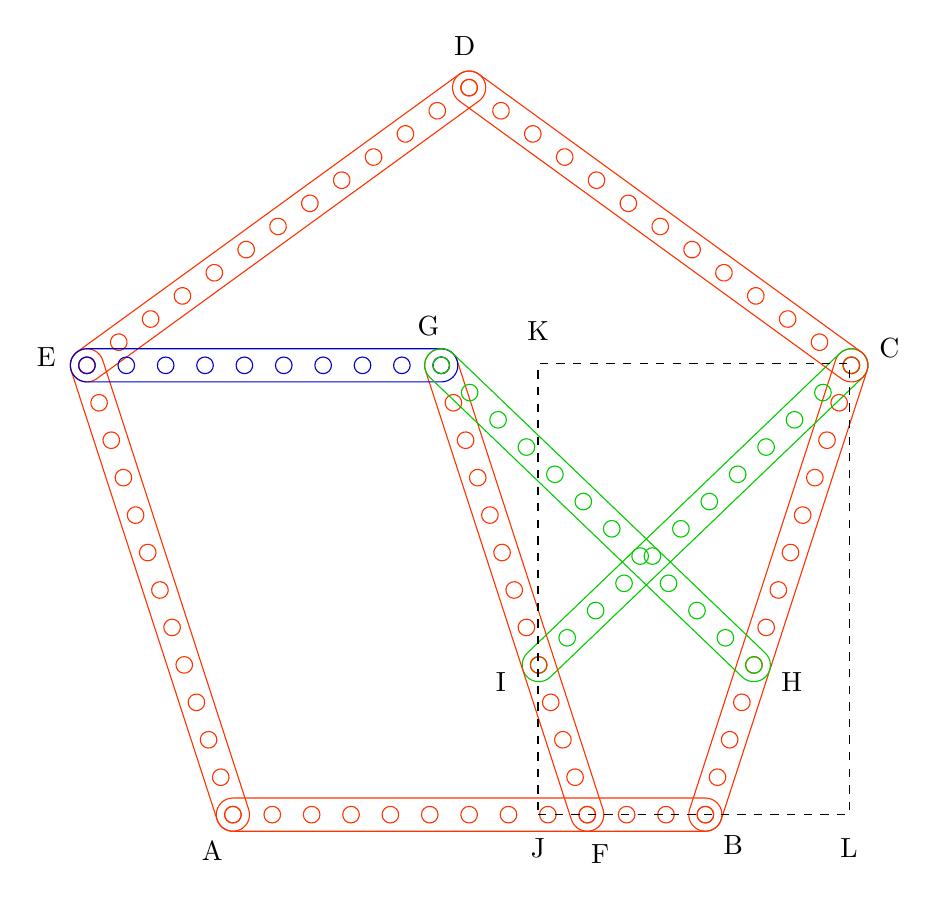
\begin{tikzpicture}

\newcommand{\rod}[4][000000] % [color][n][sep][prop]
{
 \definecolor{main}{HTML}{#1}
 \draw[main] (0,{{2*#4}})
   -- ++({#2*#3},0) arc(+90:-90:{2*#4})
   -- ++({-#2*#3},0) arc(270:90:{2*#4});
 \foreach \x in {0,1,...,#2}
  \draw[main] (\x*#3,0) circle (#4);
}

\def\s {12} \def\f {0.5} \def\p {3pt}
\def\red {FF3300} \def\blue {0000cc} \def\green {00cc00}
\begin{scope}
 \rod[\red]{\s}{\f}{\p} \path (0,0) ++(240:5*\p) node{A};
 \begin{scope}[shift={(\s*\f,0)},rotate=72]
  \rod[\red]{\s}{\f}{\p} \path (0,0) ++(240:5*\p) node{B};

  \begin{scope}[shift={(\s*\f,0)},rotate=180-28.2]
   \rod[\green]{11}{\f}{\p}
   \path (11*\f,0) ++(-20:5*\p) node{I};
  \end{scope}

  \begin{scope}[shift={(\s*\f,0)},rotate=72]
   \rod[\red]{\s}{\f}{\p} \path (0,0) ++(240:5*\p) node{C};
   \begin{scope}[shift={(\s*\f,0)},rotate=72]
    \rod[\red]{\s}{\f}{\p} \path (0,0) ++(240:5*\p) node{D};
    \begin{scope}[shift={(\s*\f,0)},rotate=72]
     \rod[\red]{\s}{\f}{\p} \path (0,0) ++(240:5*\p) node{E};
    \end{scope}
   \end{scope}
  \end{scope}
 \end{scope}

 \begin{scope}[shift={(9*\f,0)},rotate=72+36]
  \rod[\red]{\s}{\f}{\p}
  \path (0,0) ++(-180:5*\p) node{F};
  \path (\s*\f,0) ++(0:5*\p) node{G};
  \begin{scope}[shift={(\s*\f,0)},rotate=72]
   \rod[\blue]{9}{\f}{\p}
  \end{scope}
  \begin{scope}[shift={(\s*\f,0)},rotate=180+28.2]
   \rod[\green]{11}{\f}{\p}
   \path (11*\f,0) ++(20:5*\p) node{H};
  \end{scope}
 \end{scope}

\end{scope}

\def\x{7.9*\f} \def\y{11.45*\f}
\draw[dashed] (7.75*\f,0) -- ++(\x,0) -- ++(0,\y) -- ++(-\x,0) -- cycle;
\path (7.75*\f,0) ++(270:4*\p) node{J};
\path (7.75*\f,\y) ++(90:4*\p) node{K};
\path (7.75*\f+\x,0) ++(270:4*\p) node{L};
 
\end{tikzpicture}
\end{document}
